\chapter{Figures}
\label{chap:figures}

% \begin{sidewaysfigure}[p]
% 	\centering
% 	\begin{minipage}[t]{0.85\textwidth/2-1mm}
% 		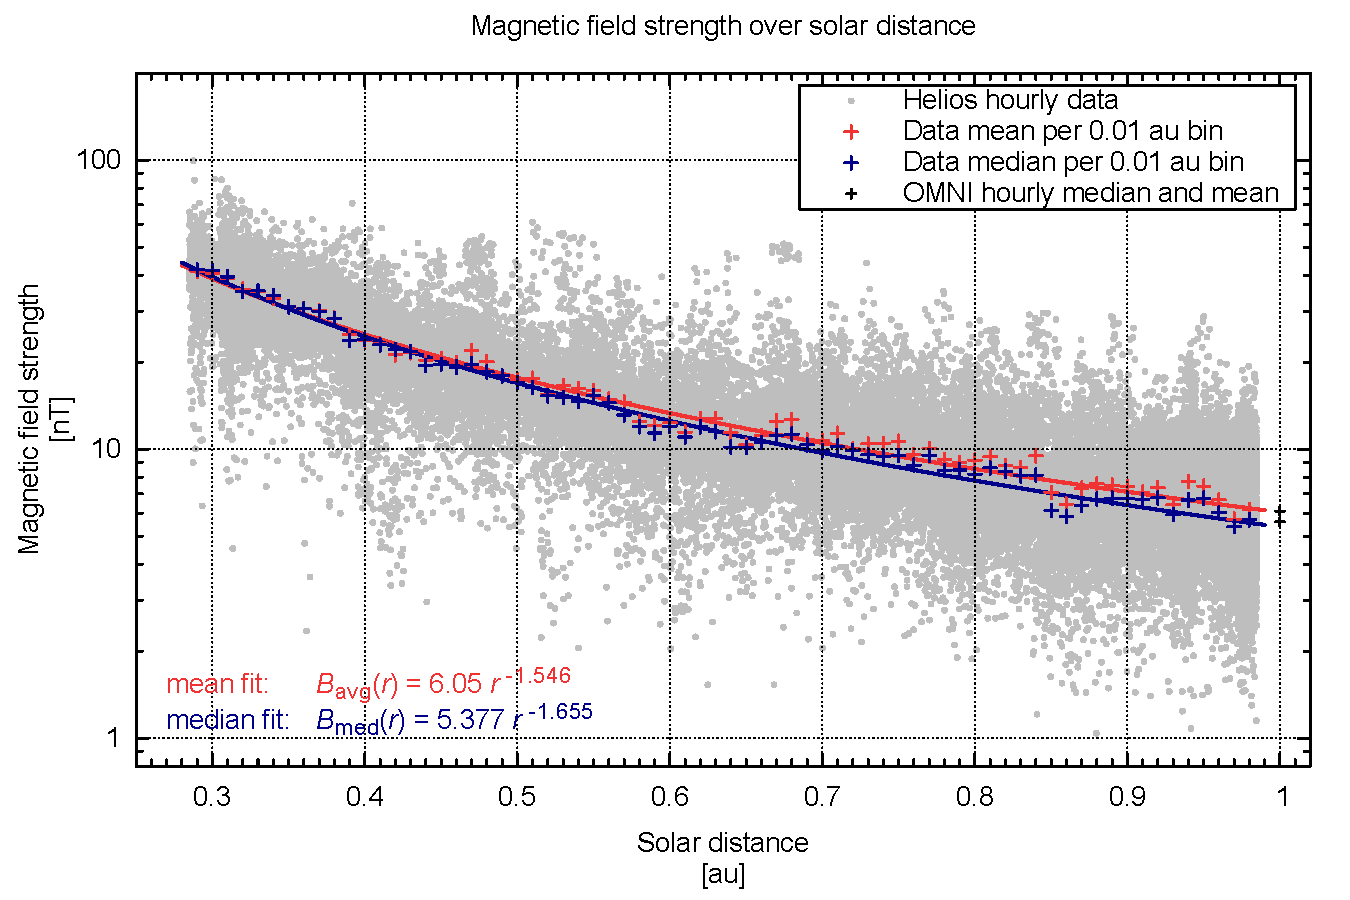
\includegraphics[width=1.0\textwidth]{images/gnuplots/radial_fit_B_thesis_pdfcairo_plot.pdf}
% 	\end{minipage}
% 	\begin{minipage}[t]{0.85\textwidth/2-1mm}
% 		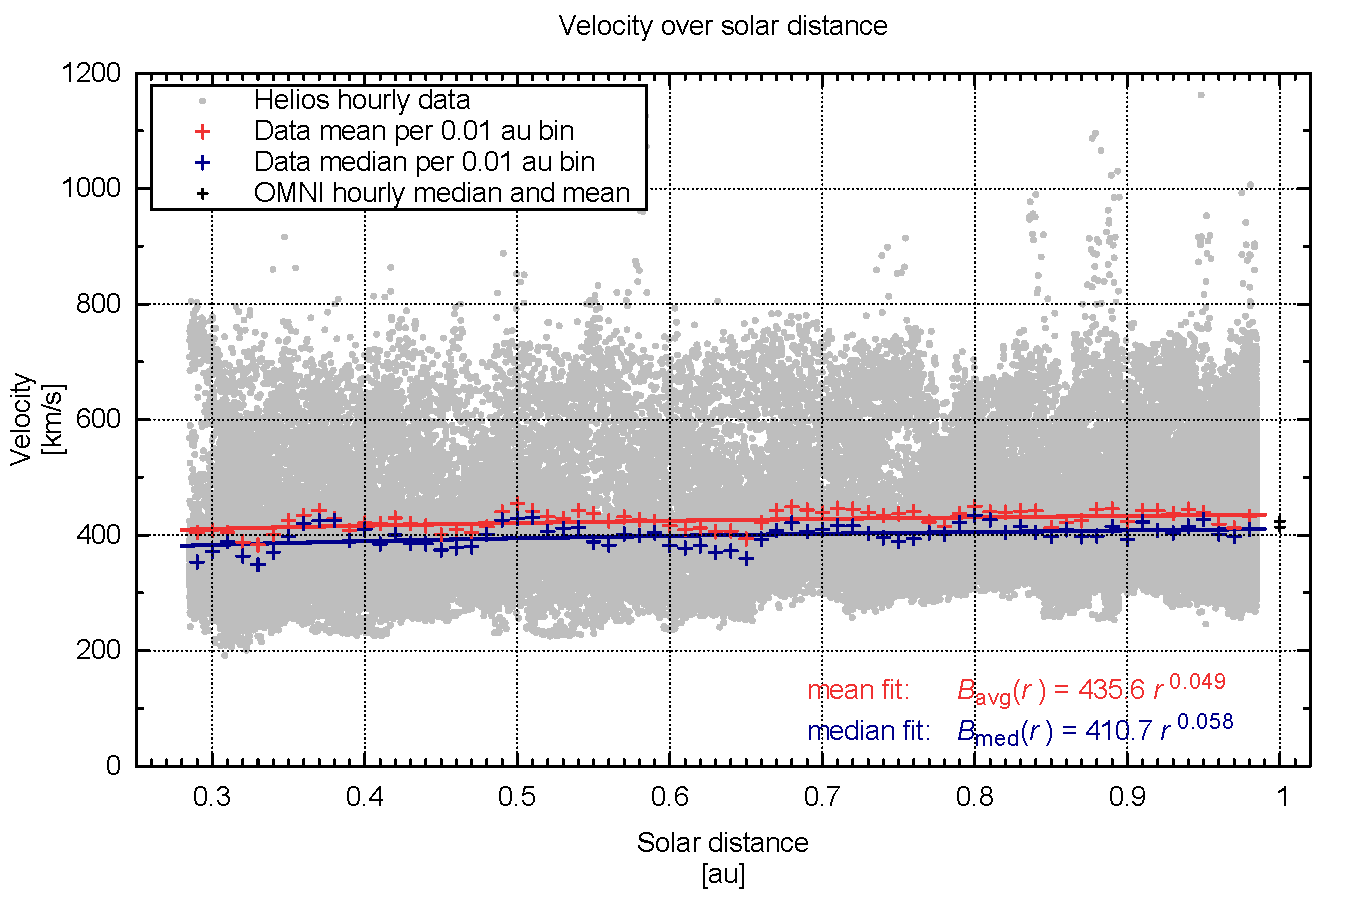
\includegraphics[width=1.0\textwidth]{images/gnuplots/radial_fit_v_thesis_pdfcairo_plot.pdf}
% 	\end{minipage}
% 	\begin{minipage}[t]{0.85\textwidth/2-1mm}
% 		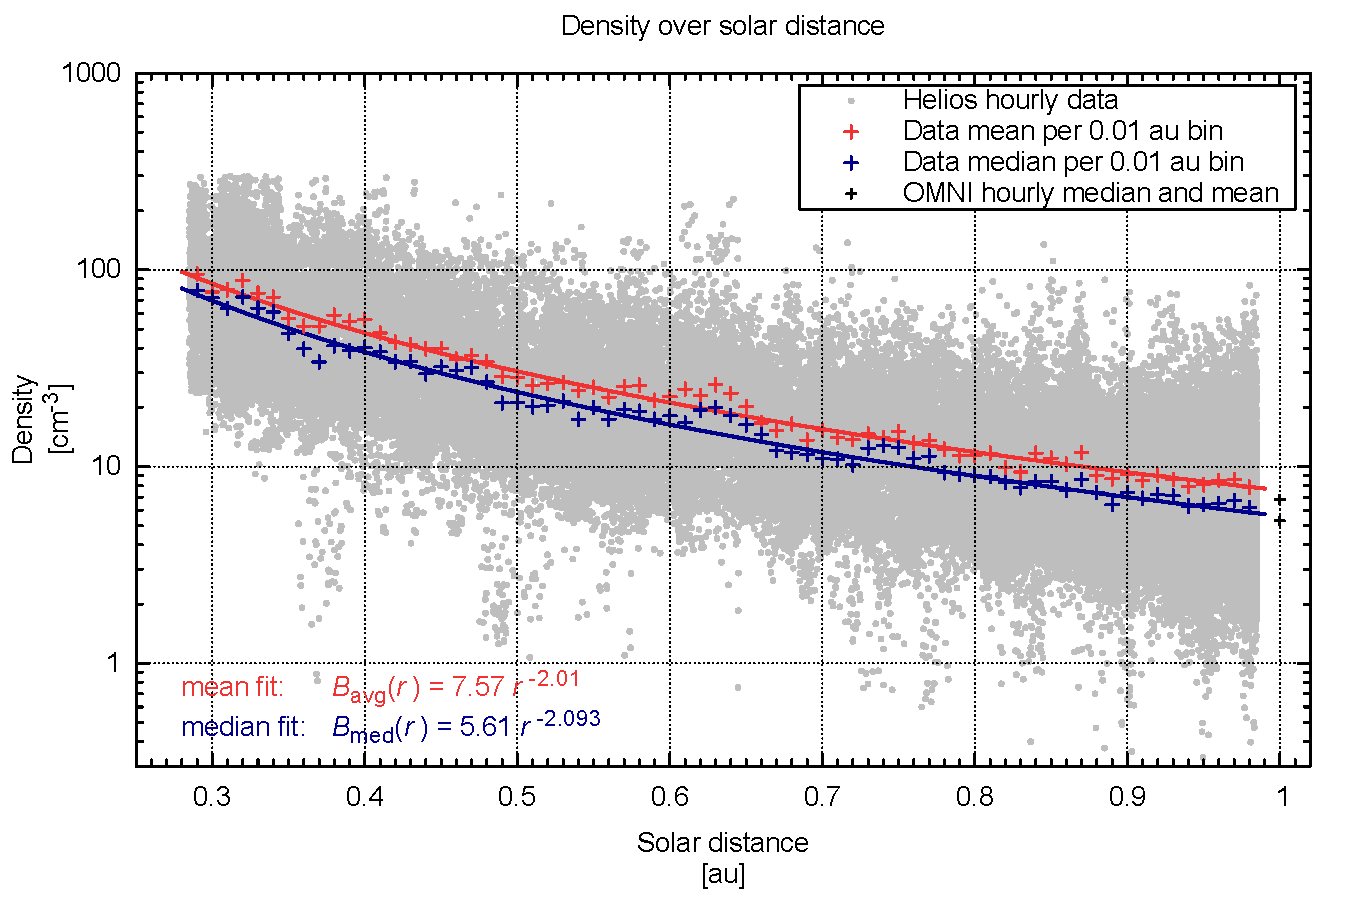
\includegraphics[width=1.0\textwidth]{images/gnuplots/radial_fit_n_thesis_pdfcairo_plot.pdf}
% 	\end{minipage}
% 	\begin{minipage}[t]{0.85\textwidth/2-1mm}
% 		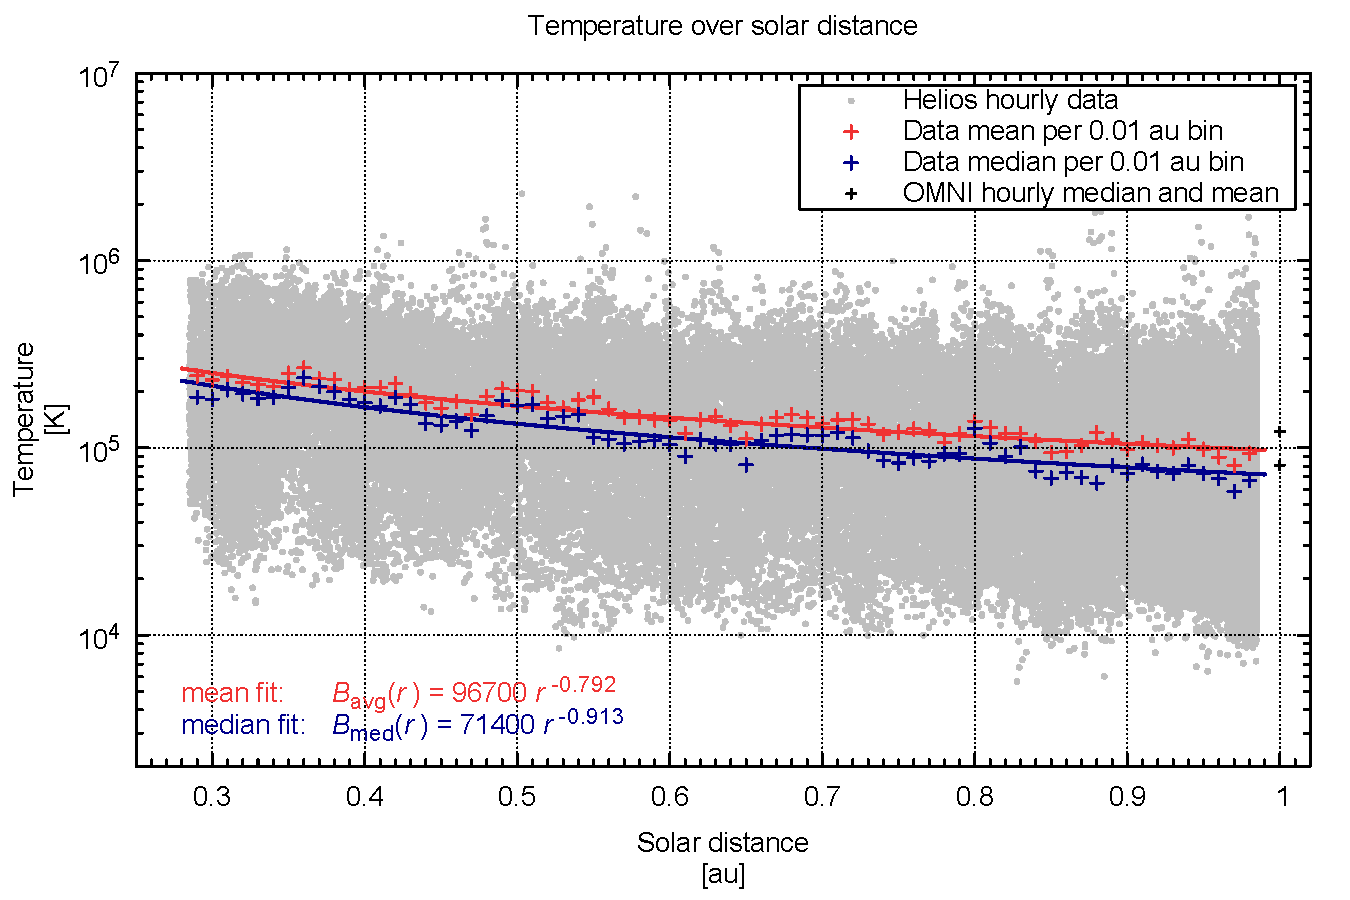
\includegraphics[width=1.0\textwidth]{images/gnuplots/radial_fit_T_thesis_pdfcairo_plot.pdf}
% 	\end{minipage}
% 	\caption{Plots of the four solar wind parameters over solar distance. The mean and median per 0.1~au data bin and their fit curves (weighted with data count) are plotted as well. Also OMNI 1~au mean and median are plotted.}
% 	\label{fig:radial_fit_4_thesis_pdfcairo_plot_minipage}
% \end{sidewaysfigure}
% 
% \begin{sidewaysfigure}[p]
% 	\centering
% 	\includegraphics[angle=10,width=0.85\textwidth]{images/gnuplots/radial_fit_4_thesis_pdfcairo_plot.pdf}
% 	\caption{Plots of the four solar wind parameters over solar distance. The mean and median per 0.1~au data bin and their fit curves (weighted with data count) are plotted as well. Also OMNI 1~au mean and median are plotted.}
% 	\label{fig:radial_fit_4_thesis_pdfcairo_plot_sideways}
% \end{sidewaysfigure}

%see Figure~\ref{fig:radial_fit_Bv_thesis_pdfcairo_plot}
\begin{figure}[p]
	\centering
	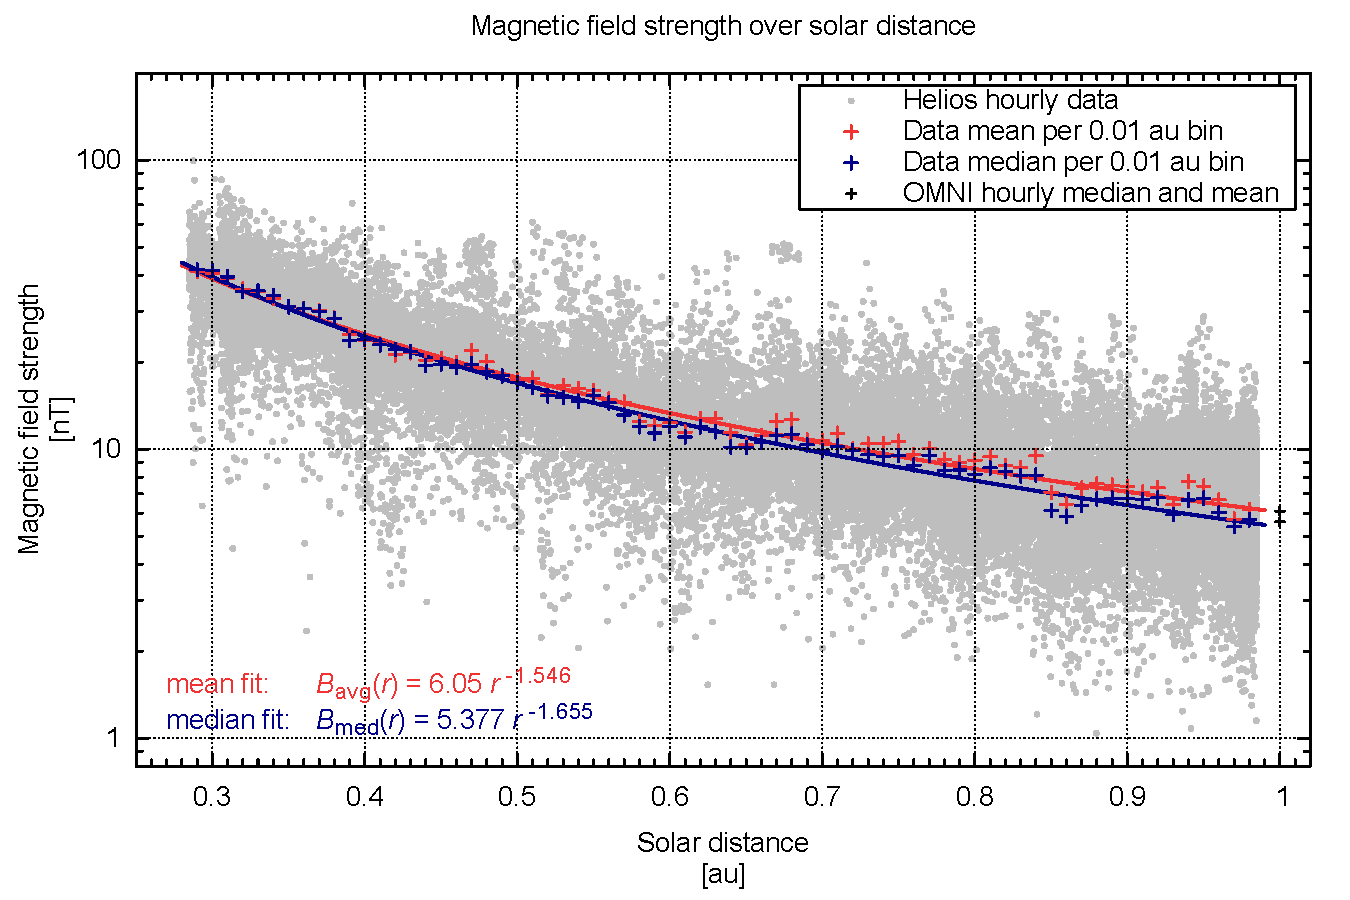
\includegraphics[width=1.0\textwidth+4mm]{images/gnuplots/radial_fit_B_thesis_pdfcairo_plot.pdf}
	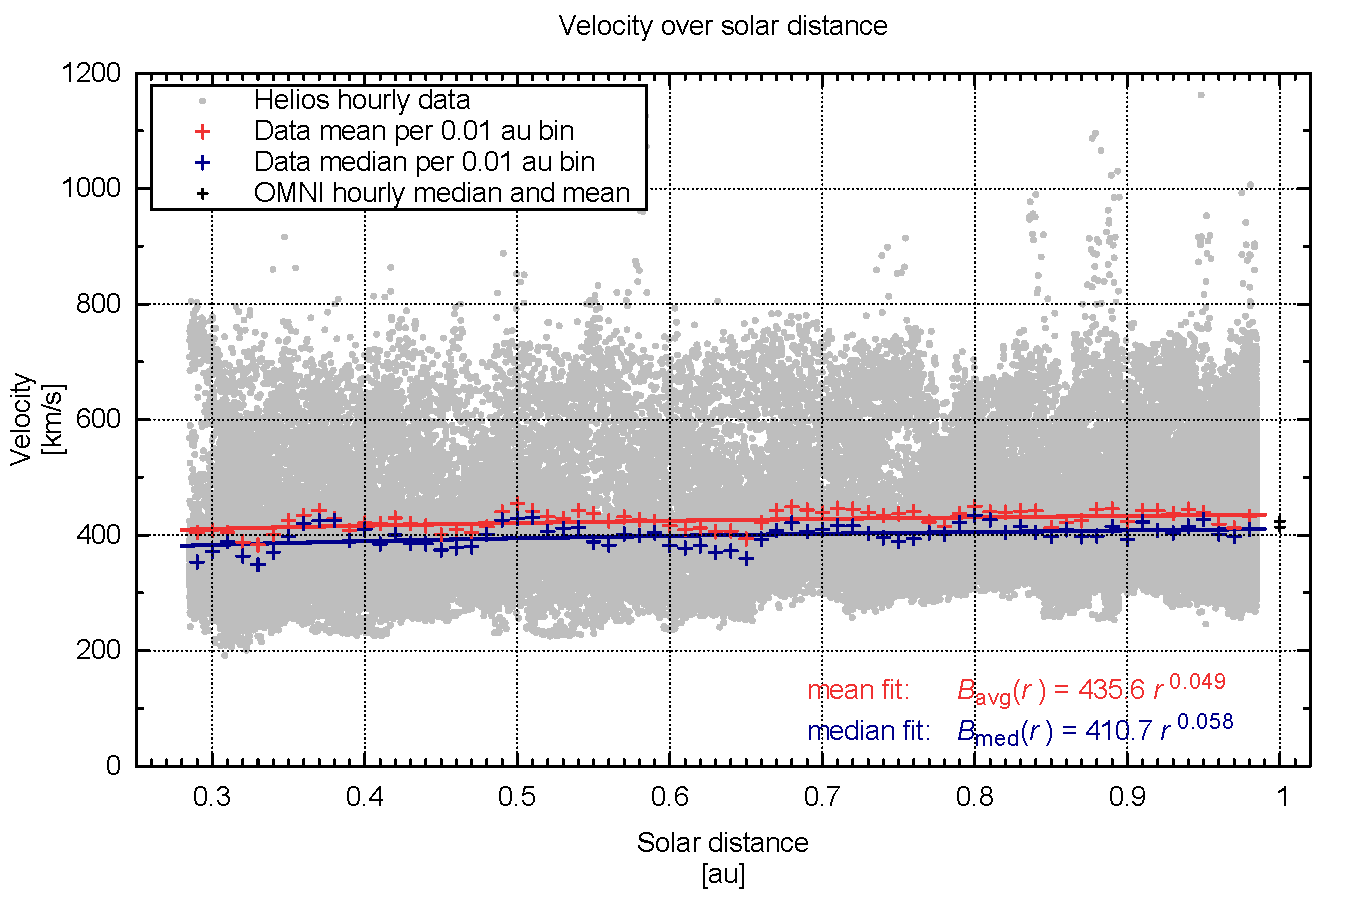
\includegraphics[width=1.0\textwidth+4mm]{images/gnuplots/radial_fit_v_thesis_pdfcairo_plot.pdf}
	\caption{Plots of the two solar wind parameters over solar distance. The mean and median per 0.1~au data bin and their fit curves (weighted with data count) are plotted as well. Also OMNI 1~au mean and median are plotted.}
	\label{fig:radial_fit_Bv_thesis_pdfcairo_plot}
\end{figure}
%see Figure~\ref{fig:radial_fit_nT_thesis_pdfcairo_plot}
\begin{figure}[p]
	\centering
	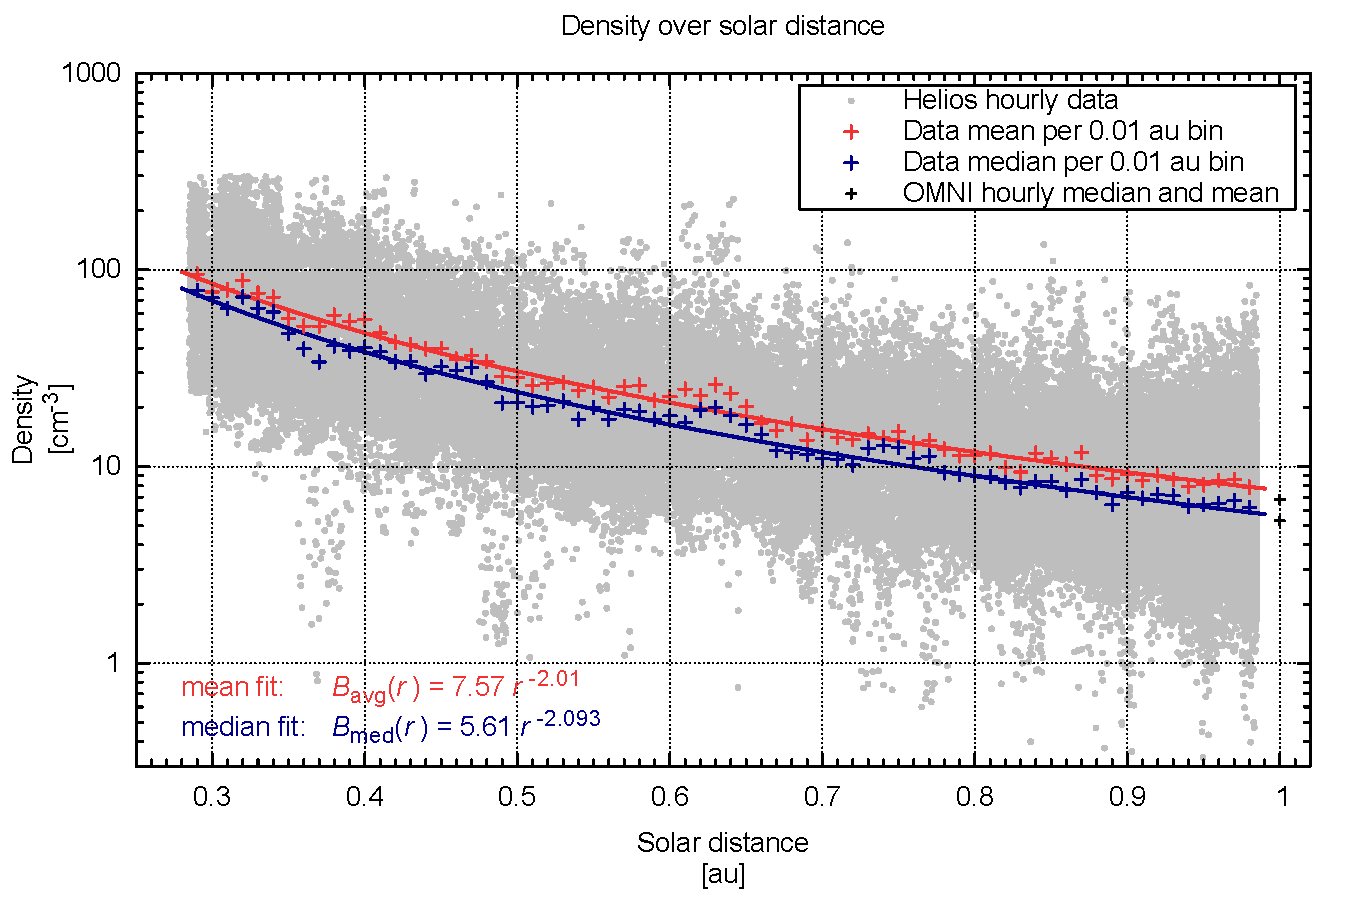
\includegraphics[width=1.0\textwidth+4mm]{images/gnuplots/radial_fit_n_thesis_pdfcairo_plot.pdf}
	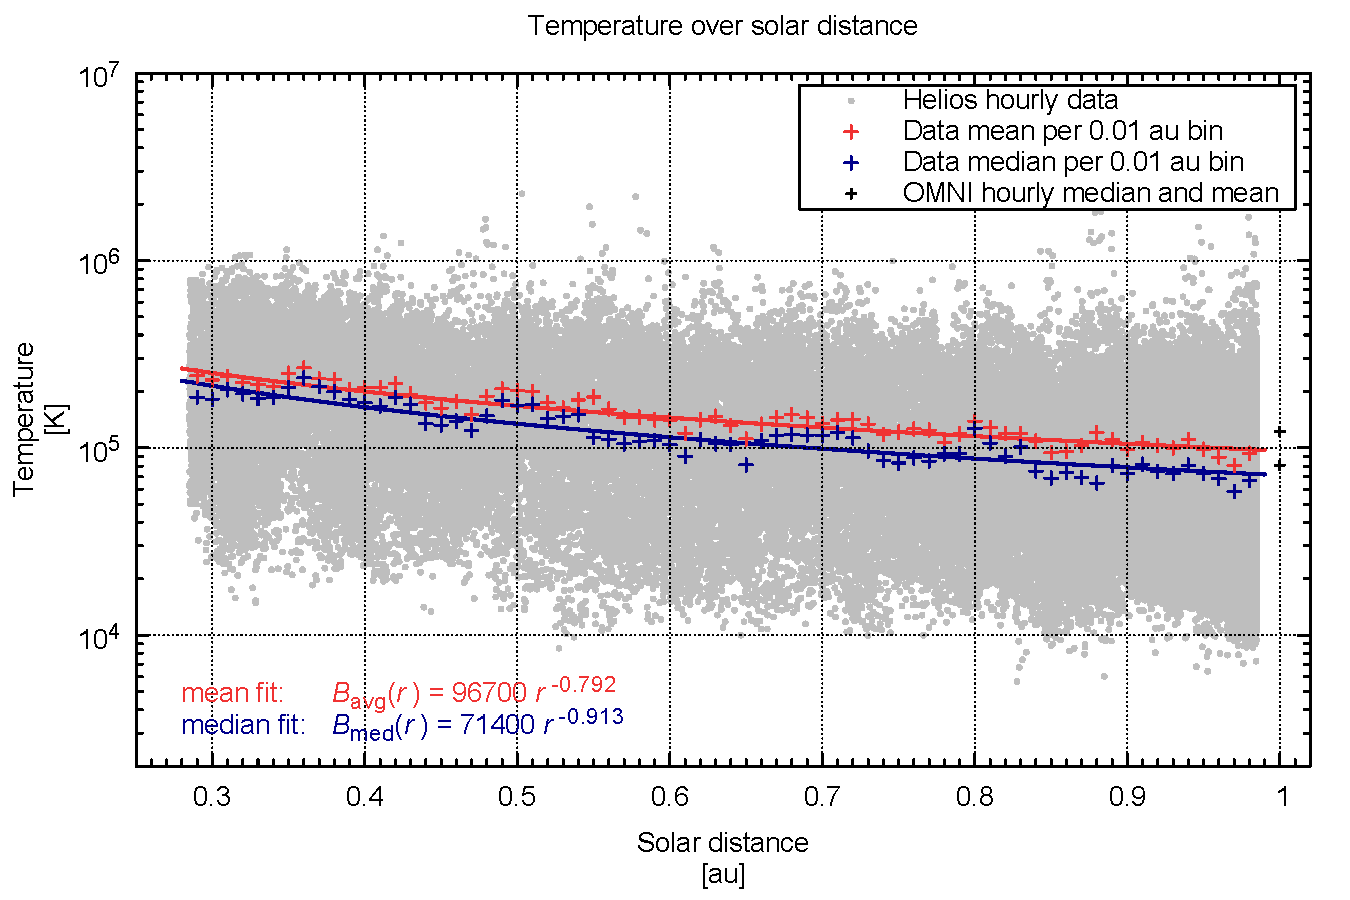
\includegraphics[width=1.0\textwidth+4mm]{images/gnuplots/radial_fit_T_thesis_pdfcairo_plot.pdf}
	\caption{Plots of the two solar wind parameters over solar distance. The mean and median per 0.1~au data bin and their fit curves (weighted with data count) are plotted as well. Also OMNI 1~au mean and median are plotted.}
	\label{fig:radial_fit_nT_thesis_pdfcairo_plot}
\end{figure}

five Helios line-up period sw plots...\\
five Helios line-up period fit curves plots...\\
